\documentclass[9pt, spanish]{entcs}

% Spanish accents
\usepackage[spanish]{babel}
\selectlanguage{spanish}
\usepackage[utf8]{inputenc}

% The mathtools package
% http://texdoc.net/texmf-dist/doc/latex/mathtools/mathtools.pdf
% https://www.codecogs.com/latex/eqneditor.php
\usepackage{mathtools}

% Algorithmic package
\usepackage{algpseudocode}
\usepackage{algorithm}
%\usepackage{algorithmic}
\usepackage{listings}

% Positioning of Figures H
\usepackage{float}

% Glossary of terms
\usepackage{glossaries}
\makeglossaries
% https://www.overleaf.com/learn/latex/Glossaries

% Búsqueda en profundidad
\newacronym{dfs}{DFS}{\textit{Depth First Search}}

\newglossaryentry{graph}
{
	name=grafo,
	description={Es una colección de puntos, llamados vértices o nodos, y segmentos de línea que conectan esos puntos, llamados aristas o arcos. Existen dos tipos de grafos, \textbf{dirigido}: es un tipo de grafo en el cual las aristas tienen un sentido definido, \textbf{no dirigido}: las aristas son relaciones simétricas y no apuntan en ningún sentido.}
}

\begin{document}
	\begin{frontmatter}
	\title{Articulation Points} 
	\author{Andrés Valencia Oliveros\thanksref{myGitHub}\thanksref{myEmail}}
	\address{Facultad de Ingeniería, Diseño e Innovación\\ 
		Institución Universitaria Politécnico Grancolombiano\\
		Bogotá, Colombia
	}
	\thanks[myGitHub]{GitHub: 
		\href{https://github.com/anvalenciao/ArticulationPoints}{\texttt{anvalenciao}}
	}
	\thanks[myEmail]{Email: 
		\href{mailto:anvalenciao@poligran.edu.co}{
			\texttt{\normalshape anvalenciao@poligran.edu.co}
		}
	}

	\renewcommand{\abstractname}{\textbf{Resumen}}
	\begin{abstract}
		\dots
	\end{abstract}

	\begin{keyword}
		articulation point, cut vertex
	\end{keyword}
\end{frontmatter}
	\section{Introducción}\label{intro}
Lorem ipsum dolor sit amet \cite{MichaelG.Paciello2000}.
	% https://books.google.com.co/books?id=m3QTSMYm5rkC&printsec=frontcover
% https://oeis.org/wiki/List_of_LaTeX_mathematical_symbols
% https://www.overleaf.com/learn/latex/Mathematical_expressions
% https://www.python-course.eu/graphs_python.php
% http://www.unipamplona.edu.co/unipamplona/portalIG/home_23/recursos/general/11072012/grafo3.pdf
% https://www.geeksforgeeks.org/difference-between-bfs-and-dfs/
% https://cs.stackexchange.com/questions/11177/how-to-check-whether-a-graph-is-connected-in-polynomial-time
% https://www.geeksforgeeks.org/difference-between-deterministic-and-non-deterministic-algorithms/
% http://www.personal.kent.edu/~rmuhamma/GraphTheory/MyGraphTheory/defEx.htm

% http://data-mining.philippe-fournier-viger.com/introduction-frequent-subgraph-mining/

% http://www.analytictech.com/networks/graphtheory.htm

% how to determine if a graph is connected

% https://es.wikipedia.org/wiki/Grafo_conexo

\section{Teoría de grafos}\label{graph theory}
En matemáticas y en ciencias de la computación, la teoría de grafos estudia las propiedades de los grafos. Un grafo \( G(V,E) \) es una colección de puntos, llamados vértices o nodos \( V = \{ v_1, v_2, \dots \} \), y segmentos de línea que conectan esos puntos, llamados aristas o arcos (en inglés \textit{edges}) \( E = \{ e_1, e_2, \dots \} \); cada arista \( e \) tiene dos \textit{\gls{endpoints}}, que son vértices. Se escribe \( u \overset{e}{-} v \), y significa que la arista \( e \) incide sobre los vértices \( u \) y \( v \); en este caso se puede decir que \( e \) conecta los vértices \( u \) y \( v \), o que los vértices \( u \) y \( v \) son \gls{adjacents} \cite{even2011graph}.

\begin{figure}[H]
	\centering
	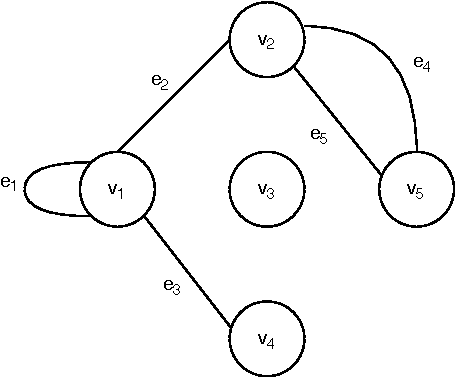
\includegraphics[width=0.35\linewidth]{document/GraphTheory/images/example-of-a-graph}
	\caption{Ejemplo de un grafo. \cite{even2011graph}}
	\label{fig:example-of-a-graph}
\end{figure}

\subsection{Grafo conexo}
Un grafo \( G \) es conexo, si por cada dos vértices \( u \) y \( v \), hay un camino (finito) que comienza en \( u \) y termina en \( v \) \cite{even2011graph}. Para verificar si un grafo \( G \) es conexo, se puede aplicar un \gls{deterministic algorithm} habitual, búsqueda en anchura en inglés \acrfull{bfs} o búsqueda en profundidad en inglés \acrfull{dfs}.

\begin{figure}[H]
	\centering
	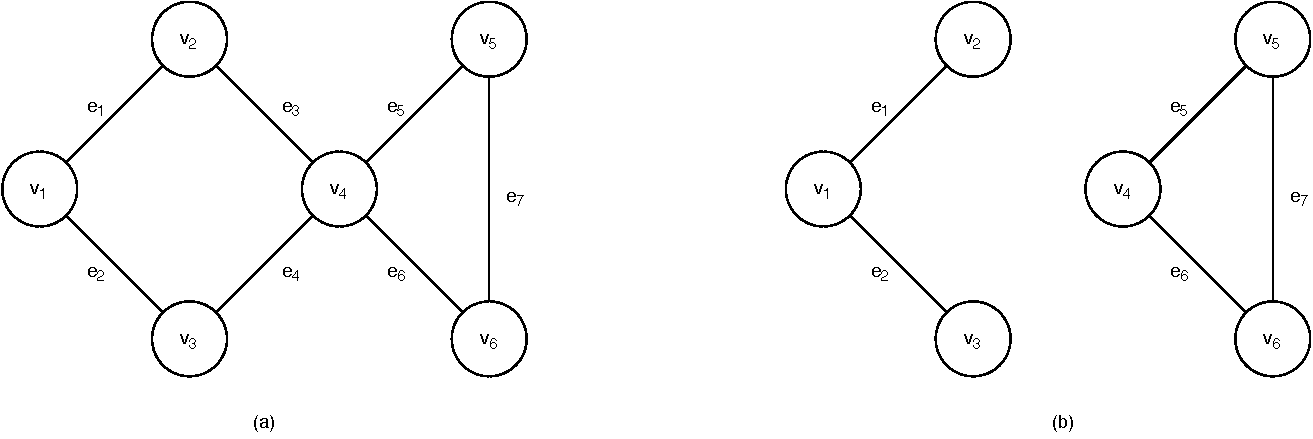
\includegraphics[width=1\linewidth]{document/GraphTheory/images/connected-disconnected-graph}
	\caption{Tipos de grafos. (a) Conexo. (b) Disconexo.}
	\label{fig:connected-disconnected-graph}
\end{figure}

% https://personales.unican.es/corcuerp/progcomp/slides/grafos.pdf
\subsection{Grafo dirigido o digrafo}
Un digrafo o grafo dirigido \( G(V,E) \) se define de manera similar a un grafo, excepto que el par de \textit{\gls{endpoints}} \( (u, v) \) de cada arista ahora está ordenado. Se escribe \( u \xrightarrow{\text{e}} v \), dónde \( u \) es el vértice inicial de \( e \); y \( v \) es el vértice final de \( e \). Se dice que la arista \( e \) está dirigida de \( u \) a \( v \) \cite{even2011graph}.

\begin{figure}[H]
	\centering
	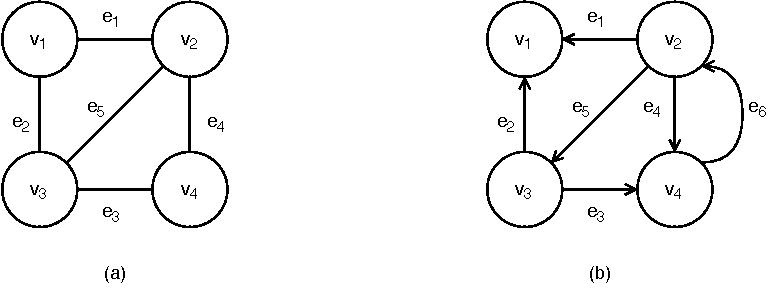
\includegraphics[width=0.6\linewidth]{document/GraphTheory/images/directed-undirected-graph}
	\caption{Tipos de grafos. (a) No dirigido. (b) Dirigido o digrafo. }
	\label{fig:directed-undirected-graph}
\end{figure}
	% graph articulation point
% https://www.geeksforgeeks.org/articulation-points-or-cut-vertices-in-a-graph/
% https://www.hackerearth.com/practice/algorithms/graphs/articulation-points-and-bridges/tutorial/
% http://www.cs.kent.edu/~aleitert/iga/slides/04ArtPointsBridges.pdf
% https://iq.opengenus.org/find-articulation-points-or-cut-vertices-in-a-graph/
% Introduction to Algorithms 3rd Edition - Page 621

% http://www.cs.kent.edu/~aleitert/iga/slides/04ArtPointsBridges.pdf
\section{Puntos de articulación}\label{articulation-points}
Un vértice \( v \) es un punto de articulación (o vértice de corte), si al eliminar el vértice \( v \) del grafo aumenta el número de componentes conectados. Es decir, genera algunos vértices inalcanzables para otros, se desconecta el grafo \cite{Jaimini2017}.

\begin{figure}[H]
	\centering
	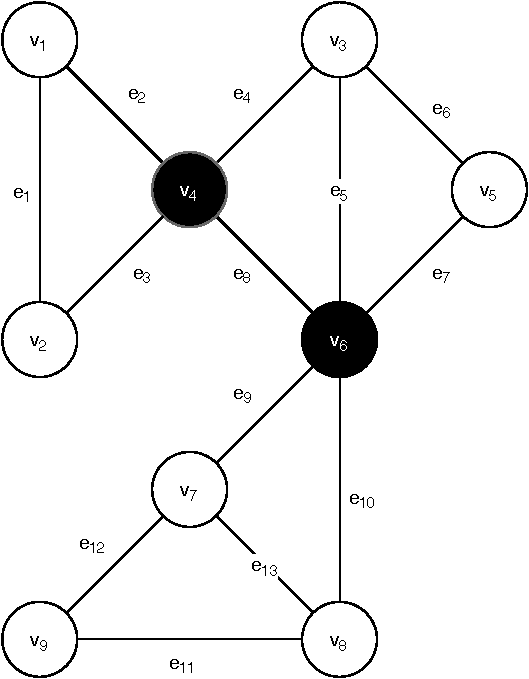
\includegraphics[width=0.4\linewidth]{document/ArticulationPoints/images/example-of-articulation-points}
	\caption{Ejemplo de grafo con dos puntos de articulación \( v_4 \) y \( v_6 \).}
	\label{fig:connected-disconnected-graph}
\end{figure}

% Encontrar los algoritmos que me permitan determinar en un grafo cuales son los nodos, en ultimas si los quito la cosa queda disconexa, una masa viscosa de puntos, otra masa viscosa de puntos, se tocan en un solo punto, el grafo es conexo, si yo quito ese nodo, entonces se partió en dos, esos puntos son claves en redes.

% https://www.geeksforgeeks.org/articulation-points-or-cut-vertices-in-a-graph/
% https://www.javamexico.org/system/files/Collections.pdf
% https://cs.stackexchange.com/questions/11177/how-to-check-whether-a-graph-is-connected-in-polynomial-time
% https://www.geeksforgeeks.org/difference-between-bfs-and-dfs/
% https://www.python-course.eu/graphs_python.php
% http://doc.sagemath.org/html/en/reference/graphs/index.html
% https://es.overleaf.com/learn/latex/algorithms
% https://math-linux.com/latex-26/faq/latex-faq/article/how-to-write-algorithm-and-pseudocode-in-latex-usepackage-algorithm-usepackage-algorithmic
% https://tex.stackexchange.com/questions/89574/language-option-supported-in-listings
% how to determine if a graph is connected
% https://github.com/mission-peace/interview/blob/master/src/com/interview/graph/ArticulationPoint.java
% https://en.wikipedia.org/wiki/Biconnected_component
% https://en.wikipedia.org/wiki/Robert_Tarjan
% https://en.wikipedia.org/wiki/Kosaraju%27s_algorithm
% https://en.wikipedia.org/wiki/Dilworth%27s_theorem

\lstdefinelanguage{JavaScript}{
	keywords={break, case, catch, continue, debugger, default, delete, do, else, finally, for, function, if, in, instanceof, new, return, switch, try, typeof, var, void, while, with},
	keywordstyle=\color{blue}\bfseries,
	ndkeywords={class, export, boolean, throw, implements, import, this},
	ndkeywordstyle=\color{cyan}\bfseries,
	identifierstyle=\color{black},
	morecomment=[l]{//},
	morecomment=[s]{/*}{*/},
	morestring=[b]',
	morestring=[b]",
	sensitive=true
}

\lstset{
	language=JavaScript,
	%extendedchars=true,
	basicstyle=\footnotesize\ttfamily,
	%showstringspaces=false,
	%showspaces=false,
	numbers=left,
	%numberstyle=\footnotesize,
	numbersep=9pt,
	tabsize=2,
	%breaklines=true,
	%showtabs=false,
	%captionpos=b
}

\renewcommand{\lstlistingname}{Algoritmo}% Listing -> Algorithm
\renewcommand{\lstlistlistingname}{Lista de \lstlistingname s}% List of Listings -> List of Algorithms


\subsection{Algoritmo de Tarjan}
El algoritmo de Tarjan se basa en una búsqueda en profundidad \acrshort{dfs}, la complejidad del tiempo de ejecución para este algoritmo es lineal, la misma del \acrshort{dfs}, \( O(V + E) \). La complejidad espacial es igual al número total de vértices \( O(V) \) \cite{Wikipedia.BiconnectedComponent}.
\subsubsection{Pseudocódigo}
\begin{algorithm}
	%\caption{Linear time depth first search}
	\begin{algorithmic}[1]
		\Function{GetArticulationPoints}{$i,d$}
			\State $visited[i] \leftarrow true$
			\State $disc[i] \leftarrow d$
			\State $low[i] \leftarrow d$
			\State $childCount \leftarrow 0$
			\State $isArticulation \leftarrow false$
			%\leq \geq \neq
			\ForAll{$ni$ \textbf{in} $adj[i]$}
				\If{not $visited[ni]$}
					\State $parent[ni] \leftarrow i$
					\State GetArticulationPoints($ni, d + 1$)
					\State $childCount \leftarrow childCount + 1$
					
					\If{$low[ni] \geq disc[i]$}
						\State $isArticulation \leftarrow true$
					\EndIf
					
					\State $low[i] \leftarrow Min(low[i], low[ni])$
					
				\ElsIf{$ni \neq parent[i]$}
					\State $low[i] \leftarrow Min(low[i], disc[ni])$
				\EndIf
			\EndFor
			
			\If{($parent[i] \neq null$ \textbf{and} $isArticulation$) \textbf{or} ($parent[i] = null$ \textbf{and} $childCount > 1$)}
				\State 
				\Return Output i as articulation point
			\EndIf
		\EndFunction
	\end{algorithmic}
\end{algorithm}

% https://medium.com/@ziyoshams/graphs-in-javascript-cc0ed170b156
\subsubsection{Implementación}
En el grafo que se muestra en la \autoref{fig:graph-dfs}, se observa la representación del mismo en un árbol \acrshort{dfs}, donde un vértice \( u \) es padre de otro vértice \( v \) y \( u \) es un punto de articulación si satisface una de las siguientes dos condiciones:
\begin{enumerate}
	\item \( u \) es la raíz del árbol DFS y tiene al menos dos hijos independientes (no están conectados entre sí).
	\item Si \( u \) no es la raíz comprueba si \( low[v] \) es mayor o igual a \( disc[u] \).
\end{enumerate}
\begin{figure}[H]
	\centering
	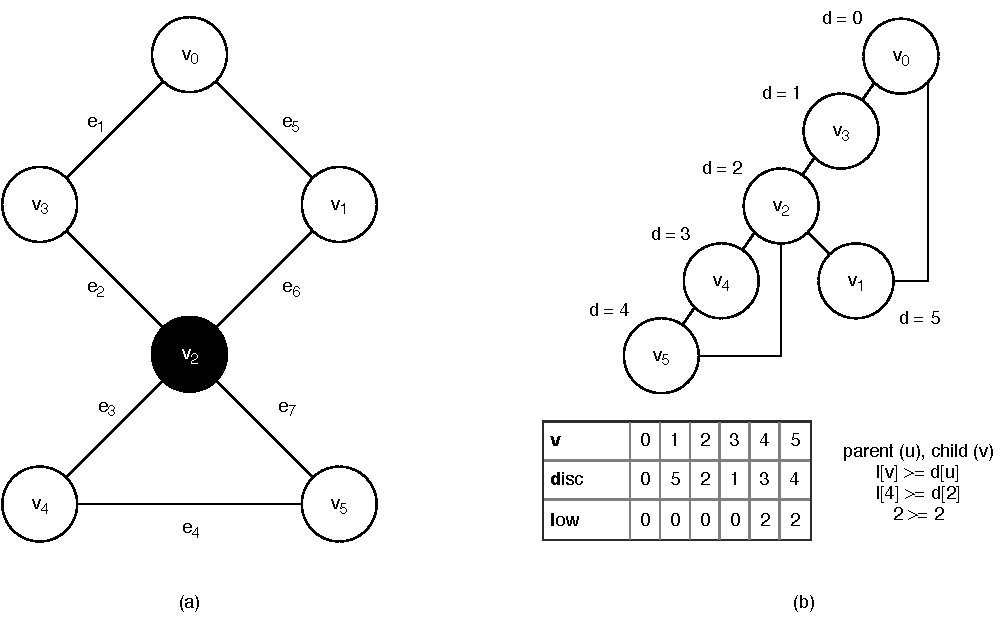
\includegraphics[width=0.8\linewidth]{document/ArticulationPoints/images/graph-dfs}
	\caption{Punto de articulación. (a) Grafo con punto de articulación en el vértice \( v_2 \). (b) Árbol DFS del grafo y \textit{Back Edge.}}
	\label{fig:graph-dfs}
\end{figure}

El siguiente código en JavaScript, es la implementación del algoritmo de Tarjan. No sé recomienda ejecutarlo en ambientes de producción, se desarrollo en este lenguaje por su facilidad de ejecutar.
\lstinputlisting[label=JSTarjan, caption=Código en JavaScript, language=JavaScript]{document/ArticulationPoints/code/Tarjan.js}

	% https://en.wikipedia.org/wiki/Cut_(graph_theory)
\section{Puentes}\label{bridges}
Una arista se llama puente si al eliminarla del grafo (manteniendo los vértices) aumenta el número de componentes conectados \cite{Jaimini2017}.

\begin{figure}[H]
	\centering
	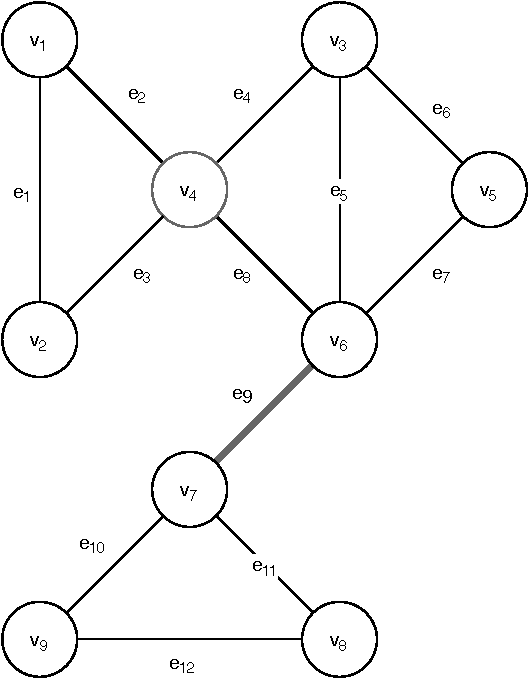
\includegraphics[width=0.4\linewidth]{document/ArticulationPoints/images/example-of-bridge}
	\caption{Ejemplo de grafo con una arista puente \( e_9 \).}
	\label{fig:connected-disconnected-graph}
\end{figure}


	\printglossary[title=Glosario de términos, toctitle=Lista de términos]
	\renewcommand{\refname}{Referencias}
\bibliographystyle{ieeetr}
\bibliography{document/Bibliography/articles}
\end{document}